
%------------------------------------------------------------------------
%
%    Copyright (C) 1985-2020  Georg Umgiesser
%
%    This file is part of SHYFEM.
%
%    SHYFEM is free software: you can redistribute it and/or modify
%    it under the terms of the GNU General Public License as published by
%    the Free Software Foundation, either version 3 of the License, or
%    (at your option) any later version.
%
%    SHYFEM is distributed in the hope that it will be useful,
%    but WITHOUT ANY WARRANTY; without even the implied warranty of
%    MERCHANTABILITY or FITNESS FOR A PARTICULAR PURPOSE. See the
%    GNU General Public License for more details.
%
%    You should have received a copy of the GNU General Public License
%    along with SHYFEM. Please see the file COPYING in the main directory.
%    If not, see <http://www.gnu.org/licenses/>.
%
%    Contributions to this file can be found below in the revision log.
%
%------------------------------------------------------------------------

Every |grd| file can be open with the |grid| program.
Normally, the coastline needs some post-processing.
It might either have a resolution that is too high, islands might show up as open lines etc..

It is important that there is one boundary line that
defines the whole domain of the computation and that must be closed. If you have a
coastline, please define your domain closing the line (including additional boundary nodes) with the gui |grid| (see
\Fig\ref{line} as example).
You can then identify what portion of the domain line will be considered open boundary.

\begin{figure}[htbp]
\centering
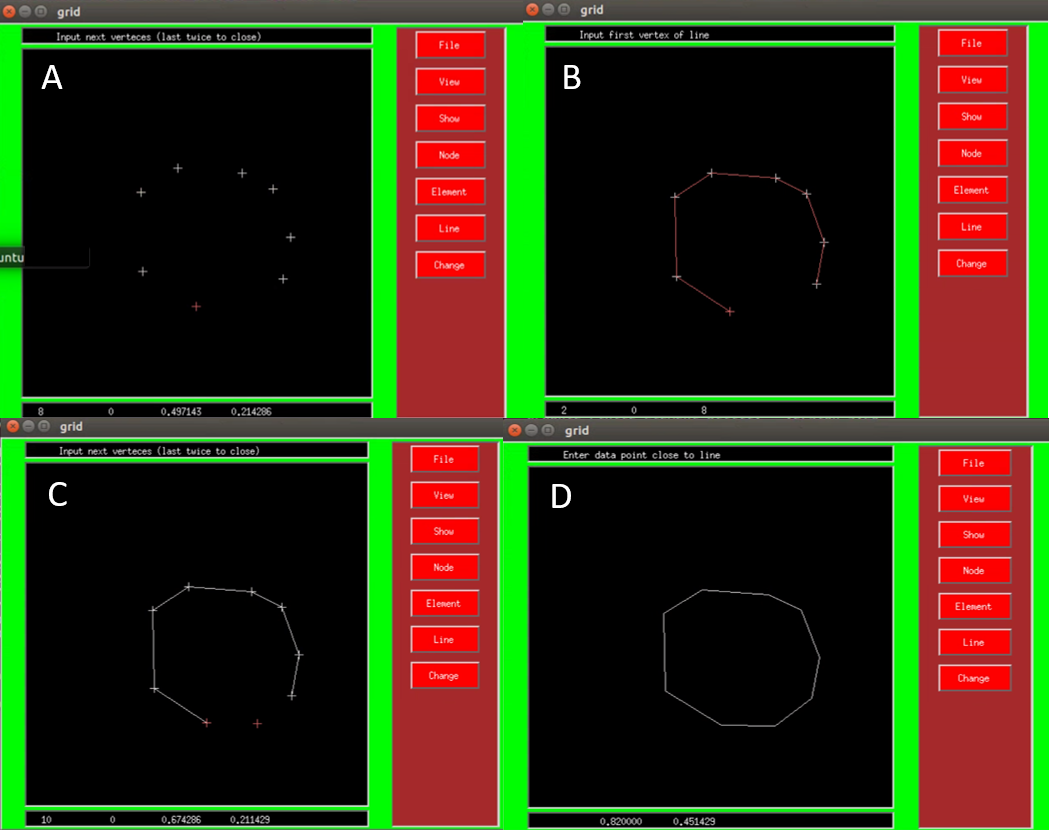
\includegraphics[scale=0.5]{crea_linea.png}
\caption{Example of the passages needed to create a closed line with the GRD GUI using commands on the right panel of the gui: A) create nodes; B) use right (to find) - left (to select) click on the mouse to chose the nodes part of the line; C) create line; D) close the line adding nodes.}
\label{line}
\end{figure}

Once this domain boundary line has been defined, care has
to be taken that the lines inside this domain, which denote
islands, are closed.

Finally, the resolution of the boundary lines (coast and islands)
have to be adjusted if you use the meshing program here provided. 
If the coastline is left as it is you might
have an excessively high resolution along the boundaries. This happens as the 
meshing algorithm does not discard any points given to it resulting in
all boundary nodes used for the meshing.
Therefore, if you have a very high resolution boundary line, you will
get many elements along the boundary and relatively little elements
(depending on the number of internal points) in the inside of the
basin.

Smoothing and reduction of the boundary lines can be done with the
routine |reduce|. The command is

\begin{code}
    reduce -s sigma -r reduct coast.grd
\end{code}

Here |sigma| specifies the length scale for the smoothing operator
and |reduct| is the length scale below which points may be deleted.
Both values have to be given in the same units of the coordinates
of the file |coast.grd|, so normally meters.
The smoothed file can be found in |smooth.grd| and the subsequently
reduced file in |reduct.grd|. 

If there are some points in the boundary line that should not be smoothed
they can be given a depth value of -1. This is a flag that indicates
that the position of these points will not be touched.


